\documentclass[a4paper,11pt]{article}
\usepackage[T1]{fontenc}
\usepackage{lmodern}
\usepackage{babel}
\babelprovide[main,import]{spanish}
\usepackage[margin=2.4cm,headheight=14pt]{geometry}
\usepackage{microtype}
\usepackage{graphicx,xcolor,booktabs,array,tabularx,enumitem,float}
\usepackage[font=small,skip=6pt]{caption}
\usepackage{tikz}
\usetikzlibrary{positioning,arrows.meta}
\usepackage{fancyhdr}
\usepackage[hidelinks]{hyperref}

\definecolor{navy}{HTML}{263951}
\definecolor{greytext}{HTML}{475568}
\definecolor{panel}{HTML}{EFF3F7}
\hypersetup{
  pdftitle={SolarBell - Manual del sistema},
  pdfauthor={Andrés Felipe Ortiz Rodríguez, Néstor Junior Hernández López, José Enrique Otero Pineda, Julián Camilo Doria Guevara},
  pdfsubject={Manual técnico del Proyecto de Aula Semestral},
  bookmarksopen=true
}
\addto\captionsspanish{%
  \renewcommand{\contentsname}{Índice}%
  \renewcommand{\figurename}{Figura}%
  \renewcommand{\tablename}{Tabla}%
}
\setcounter{tocdepth}{1}
\setlength{\parskip}{5pt plus 1pt}
\setlength{\parindent}{0pt}
\setlength{\emergencystretch}{2em}
\renewcommand{\arraystretch}{1.19}
\setlist{topsep=3pt,itemsep=4pt,parsep=0pt,leftmargin=*}
\raggedbottom
\newcolumntype{Y}{>{\raggedright\arraybackslash}X}
\newcolumntype{P}[1]{>{\raggedright\arraybackslash}p{#1}}
\newcommand{\pin}[1]{\texttt{#1}}
\newcommand{\fuente}[1]{\par\smallskip{\centering\footnotesize #1\par}}
\newcommand{\nota}[1]{%
  \par\smallskip\noindent{\setlength{\fboxsep}{9pt}%
  \colorbox{panel}{\parbox{\dimexpr\linewidth-2\fboxsep\relax}{\small #1}}}%
  \par\smallskip
}
\pagestyle{fancy}
\fancyhf{}
\fancyhead[L]{\small\color{greytext}SolarBell}
\fancyhead[R]{\small\color{greytext}Manual del sistema}
\fancyfoot[C]{\small\thepage}
\renewcommand{\headrulewidth}{0.35pt}
\tikzset{
  bloque/.style={draw=navy,fill=panel,rounded corners=2pt,minimum height=10mm,align=center,font=\small,text width=2.64cm,inner sep=4pt},
  enlace/.style={-{Stealth[length=2.3mm]},draw=navy,semithick},
  rotulo/.style={font=\footnotesize,fill=white,inner sep=2pt,text=greytext}
}

\begin{document}
\begin{titlepage}
  \centering
  \vspace*{1.15cm}
  {\large\bfseries UNIVERSIDAD DE CÓRDOBA\par}
  \vspace{0.24cm}
  {\bfseries FACULTAD DE INGENIERÍA\par}
  \vspace{0.20cm}
  {\bfseries PROGRAMA DE INGENIERÍA DE SISTEMAS\par}
  \vspace{0.20cm}
  {\bfseries SEDE MONTERÍA\par}
  \vfill
  {\large\bfseries PROYECTO DE AULA SEMESTRAL\par}
  \vspace{0.9cm}
  {\Huge\bfseries\color{navy} Manual del sistema\par}
  \vspace{0.25cm}
  {\LARGE\bfseries SolarBell\par}
  \vspace{0.38cm}
  {\large Sistema de timbre automatizado con energía solar\par}
  \vspace{0.7cm}
  {\color{greytext}Instalación documentada\par
  Institución Educativa Cecilia de Lleras, Montería\par}
  \vfill
  {\bfseries Presentado por\par}
  \vspace{0.28cm}
  Andrés Felipe Ortiz Rodríguez\par
  Néstor Junior Hernández López\par
  José Enrique Otero Pineda\par
  Julián Camilo Doria Guevara\par
  \vfill
  {\bfseries Docentes\par}
  \vspace{0.27cm}
  Antonio Fernando Movilla Quintero\par
  Milton Eduardo Hernández Zakzuk\par
  \vfill
  {\bfseries Arquitectura del Computador y Sistemas Operativos\par}
  \vspace{0.28cm}
  Montería, noviembre de 2026\par
  \vspace*{0.2cm}
\end{titlepage}

\pagenumbering{arabic}
\tableofcontents

\section{Alcance y responsabilidades}
Este manual describe el sistema SolarBell instalado en la Institución Educativa Cecilia de Lleras, en Montería. Está dirigido a quienes administran el equipo y a quienes prestan soporte técnico. Incluye las interfaces del prototipo, la configuración inicial, la carga del firmware, las comprobaciones de servicio y el diagnóstico de fallas. Corresponde al firmware 0.8.0 y a la aplicación Android de la rama \pin{main}, revisión \pin{0adeb14} \cite{informe,fichas,diagrama,repo}.

\begin{table}[H]
\centering\small
\caption{Responsabilidades por tipo de intervención}
\begin{tabularx}{\linewidth}{@{}P{4cm}Y@{}}
\toprule
\textbf{Responsable} & \textbf{Intervención} \\
\midrule
Personal autorizado del colegio & Administra el horario desde Android, revisa el historial y coordina las pruebas sonoras. Reporta las anomalías. \\
Soporte del sistema & Identifica la versión del firmware, comprueba conectividad, reloj y programación, y conserva el registro de cambios. \\
Personal competente en electrotecnia & Revisa la alimentación, los medios de aislamiento, las protecciones y la conmutación de la campana. Autoriza la intervención y la puesta en servicio eléctrica según corresponda. \\
\bottomrule
\end{tabularx}
\end{table}

\nota{\textbf{Antes de abrir el equipo.} El sistema tiene alimentación fotovoltaica con batería, una salida de 110\,V del inversor y una ruta de 110\,V desde la red escolar. La ruta de la red escolar puede permanecer energizada con el ESP32 y la radio Wi-Fi apagados. El personal competente debe aislar todas las fuentes pertinentes, impedir su reconexión y verificar la ausencia de tensión antes de intervenir, siguiendo el procedimiento de trabajo sin tensión aplicable \cite{retie}.}

Para el uso diario, consulte la Sección~\ref{sec:servicio}. Si el timbre se activa fuera de horario, consulte la Sección~\ref{sec:diagnostico} y suspenda las pruebas hasta identificar el origen del aviso.

\clearpage
\section{Arquitectura y modos de operación}
\label{sec:arquitectura}
\subsection{Recorrido de la energía y del control}
El panel carga la batería a través del controlador PWM. La salida de carga de 12\,V del controlador alimenta el regulador de 5\,V y la rama del inversor. El ESP32 consulta el reloj DS3231SN y controla los dos canales de relé. La aplicación se conecta al ESP32 por HTTP en una red Wi-Fi local \cite{fichas,diagrama}.

\begin{figure}[H]
\centering
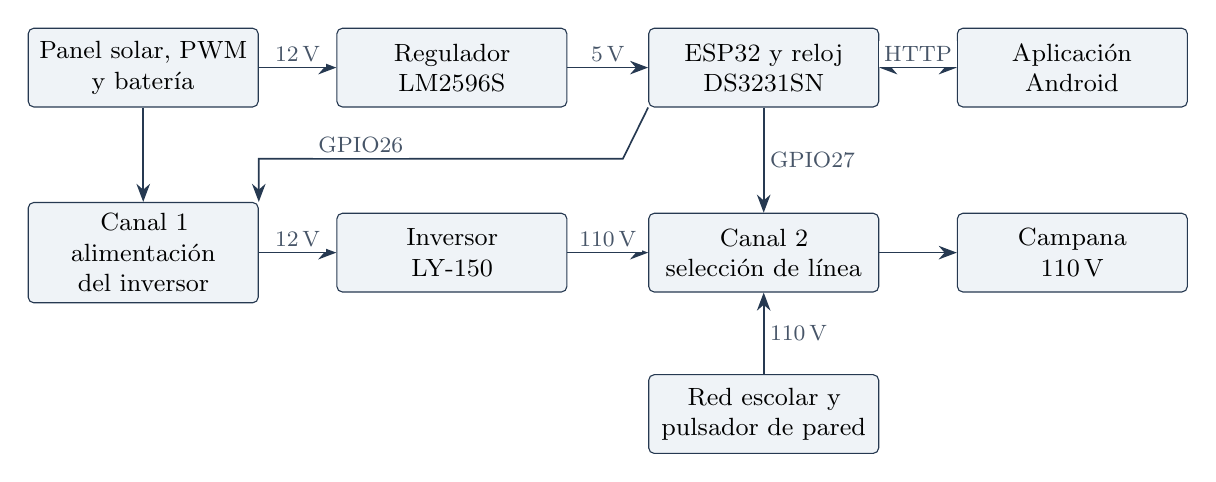
\begin{tikzpicture}
  \node[bloque] (solar) at (-5.9,2.35) {Panel solar, PWM\par y batería};
  \node[bloque] (reductor) at (-1.98,2.35) {Regulador\par LM2596S};
  \node[bloque] (esp) at (1.98,2.35) {ESP32 y reloj\par DS3231SN};
  \node[bloque] (app) at (5.9,2.35) {Aplicación\par Android};
  \node[bloque] (rele1) at (-5.9,0.00) {Canal 1\par alimentación del inversor};
  \node[bloque] (inv) at (-1.98,0.00) {Inversor\par LY-150};
  \node[bloque] (rele2) at (1.98,0.00) {Canal 2\par selección de línea};
  \node[bloque] (campana) at (5.9,0.00) {Campana\par 110\,V};
  \node[bloque] (red) at (1.98,-2.05) {Red escolar y\par pulsador de pared};
  \draw[enlace] (solar) -- node[above,rotulo] {12\,V} (reductor);
  \draw[enlace] (reductor) -- node[above,rotulo] {5\,V} (esp);
  \draw[enlace,{Stealth[length=2.3mm]}-{Stealth[length=2.3mm]}] (esp) -- node[above,rotulo] {HTTP} (app);
  \draw[enlace] (solar) -- (rele1);
  \draw[enlace] (esp.south) -- node[right,rotulo] {GPIO27} (rele2.north);
  \draw[enlace] (esp.south west) -- ++(-.32,-.65) -| node[pos=.36,above,rotulo] {GPIO26} (rele1.north east);
  \draw[enlace] (rele1) -- node[above,rotulo] {12\,V} (inv);
  \draw[enlace] (inv) -- node[above,rotulo] {110\,V} (rele2);
  \draw[enlace] (red) -- node[right,rotulo] {110\,V} (rele2);
  \draw[enlace] (rele2) -- (campana);
\end{tikzpicture}
\caption{Relación funcional entre alimentación, control y campana}
\end{figure}

\begin{table}[H]
\centering\small
\caption{Condiciones de operación}
\begin{tabularx}{\linewidth}{@{}P{3.4cm}YY@{}}
\toprule
\textbf{Modo} & \textbf{Origen} & \textbf{Respuesta esperada} \\
\midrule
Programado & Coincidencia del RTC con un evento guardado. & El ESP32 ejecuta los toques, sus duraciones y las pausas. \\
Inmediato desde Android & Orden enviada desde el teléfono conectado. & El ESP32 ejecuta el patrón indicado. La app puede solicitar detener el toque en curso. \\
Pulsador de pared & Pulsación con red escolar disponible y canal 2 en reposo. & La campana recibe la alimentación de la red por la ruta manual. \\
Ahorro de radio con red del colegio & Interruptor de Wi-Fi cerrado y red del colegio guardada. & Se apaga la red SolarBell y la radio duerme entre balizas del router. La app solo funciona desde la red del colegio y puede tardar unos cientos de milisegundos más en responder. \\
Wi-Fi apagado & Interruptor de Wi-Fi cerrado sin red del colegio guardada. & El ESP32 continúa ejecutando el horario guardado si tiene alimentación. La app pierde el enlace. \\
\bottomrule
\end{tabularx}
\end{table}

En un timbrado gobernado por el ESP32, el canal 1 alimenta el inversor durante la secuencia completa. El firmware espera 2\,s a que el inversor arranque antes del primer repique. El canal 2 aplica la línea del inversor en cada repique y vuelve a reposo en las pausas. Al finalizar la secuencia, el canal 1 corta la alimentación del inversor y el ESP32 anota el toque en su historial \cite{fichas,diagrama,repo}.

En las tres situaciones del interruptor, el horario se ejecuta igual. El interruptor solo cambia qué redes quedan disponibles. La red SolarBell en modo punto de acceso consume del orden de 100\,mA todo el día, unos 2,4\,Ah diarios frente a los 7,5\,Ah de la batería, por lo que el modo de ahorro conviene en temporadas de poco sol \cite{repo}.

\clearpage
\section{Hardware y señales documentadas}
\label{sec:hardware}
\subsection{Identificación de componentes}
Use los modelos y valores nominales para identificar los componentes del prototipo. Para un reemplazo, el personal técnico comprueba compatibilidad eléctrica, corriente de arranque, tipo de carga y requisitos de protección de la instalación \cite{fichas,diagrama}.

\begin{table}[H]
\centering\small
\caption{Componentes del montaje final}
\begin{tabularx}{\linewidth}{@{}P{3.14cm}P{5.7cm}Y@{}}
\toprule
\textbf{Elemento} & \textbf{Modelo o valor documentado} & \textbf{Función} \\
\midrule
Panel solar & Powest SZYL-P30-18C, 30\,Wp & Generación fotovoltaica. \\
Controlador y batería & PWM 12\,V / 10\,A y VRLA FuliBattery FL1275GS, 12\,V / 7,5\,Ah & Carga y reserva de energía. \\
Regulador & LM2596S de 12\,V a 5\,V & Alimentación regulada del control. \\
Controlador y RTC & ESP32 DevKit v1 y HW-084 DS3231SN & Gestión de horario e interfaces y referencia de fecha y hora. \\
Módulo de relés & Módulo optoacoplado de dos canales, bobinas de 5\,V, marcado de 10\,A & Alimentación del inversor y conmutación de la campana. \\
Inversor y campana & LY-150 de 150\,W, salida de 110\,V a 60\,Hz. Campana de 110\,V. & Conversión CC--CA y aviso sonoro. \\
Mandos físicos & Pulsador EXE de 110\,V e interruptor basculante de dos terminales & Toque desde la red escolar y control de la radio Wi-Fi. \\
Estabilización y protección & Condensador de 1000\,\(\mu\)F / 16\,V, diodo 1N4007 y varistor 14D241K & Estabilización de 5\,V y supresión de transitorios según el diagrama. \\
\bottomrule
\end{tabularx}
\end{table}

\subsection{Mapa de señales del ESP32}
\begin{table}[H]
\centering\small
\caption{Correspondencias según el diagrama final}
\begin{tabularx}{\linewidth}{@{}P{3.05cm}P{5cm}Y@{}}
\toprule
\textbf{Terminal} & \textbf{Destino documentado} & \textbf{Función} \\
\midrule
\pin{GPIO21} & \pin{SDA} del RTC & Datos del bus I\textsuperscript{2}C. \\
\pin{GPIO22} & \pin{SCL} del RTC & Reloj del bus I\textsuperscript{2}C. \\
\pin{GPIO26} & \pin{IN1} del módulo de relés & Mando del canal 1 para el inversor. \\
\pin{GPIO27} & \pin{IN2} del módulo de relés & Mando del canal 2 para la campana. \\
\pin{GPIO33}, \pin{GND} & Interruptor basculante de Wi-Fi & Entrada con resistencia de \textit{pull-up} interna. Abierto o sin cable: red SolarBell activa. Cerrado: modo de ahorro. \\
\pin{GPIO2} & LED azul de la placa & Indicador de estado (Tabla~\ref{tab:led}). \\
\pin{VIN}, \pin{GND} & Salida de 5\,V del LM2596S & Alimentación y referencia del control. \\
\pin{3V3}, \pin{GND} & \pin{VCC} y \pin{GND} del RTC & Alimentación y referencia del reloj. \\
\bottomrule
\end{tabularx}
\end{table}

El diagrama indica un puente entre \pin{JD-VCC} y \pin{VCC} en el módulo de relés. Los pines de los relés y del interruptor se fijan en \pin{configuracion.h} al compilar (sección~\ref{sec:firmware}); los valores de la tabla son los de la instalación. Verifique las etiquetas de la unidad intervenida antes de sustituir una placa.

\begin{table}[H]
\centering\small
\caption{Lectura del LED azul de la placa}
\label{tab:led}
\begin{tabularx}{\linewidth}{@{}P{4cm}Y@{}}
\toprule
\textbf{LED} & \textbf{Significado} \\
\midrule
Parpadeo lento & El equipo no tiene hora y no ejecuta el horario hasta que un teléfono se conecte. \\
Dos destellos cortos & Se unió un teléfono o se guardó el horario. \\
Encendido fijo & Toque en curso. Se apaga durante cada pausa. \\
\bottomrule
\end{tabularx}
\end{table}

\clearpage
\subsection{Esquema eléctrico de referencia}
\label{sec:esquema}
La Figura~\ref{fig:esquema} reproduce el circuito final del proyecto. La ficha técnica identifica el panel y el interruptor de Wi-Fi como elementos adicionales que no aparecen dibujados en el esquema. El interruptor va entre \pin{GPIO33} y \pin{GND} \cite{fichas,diagrama,repo}.

\begin{figure}[H]
\centering
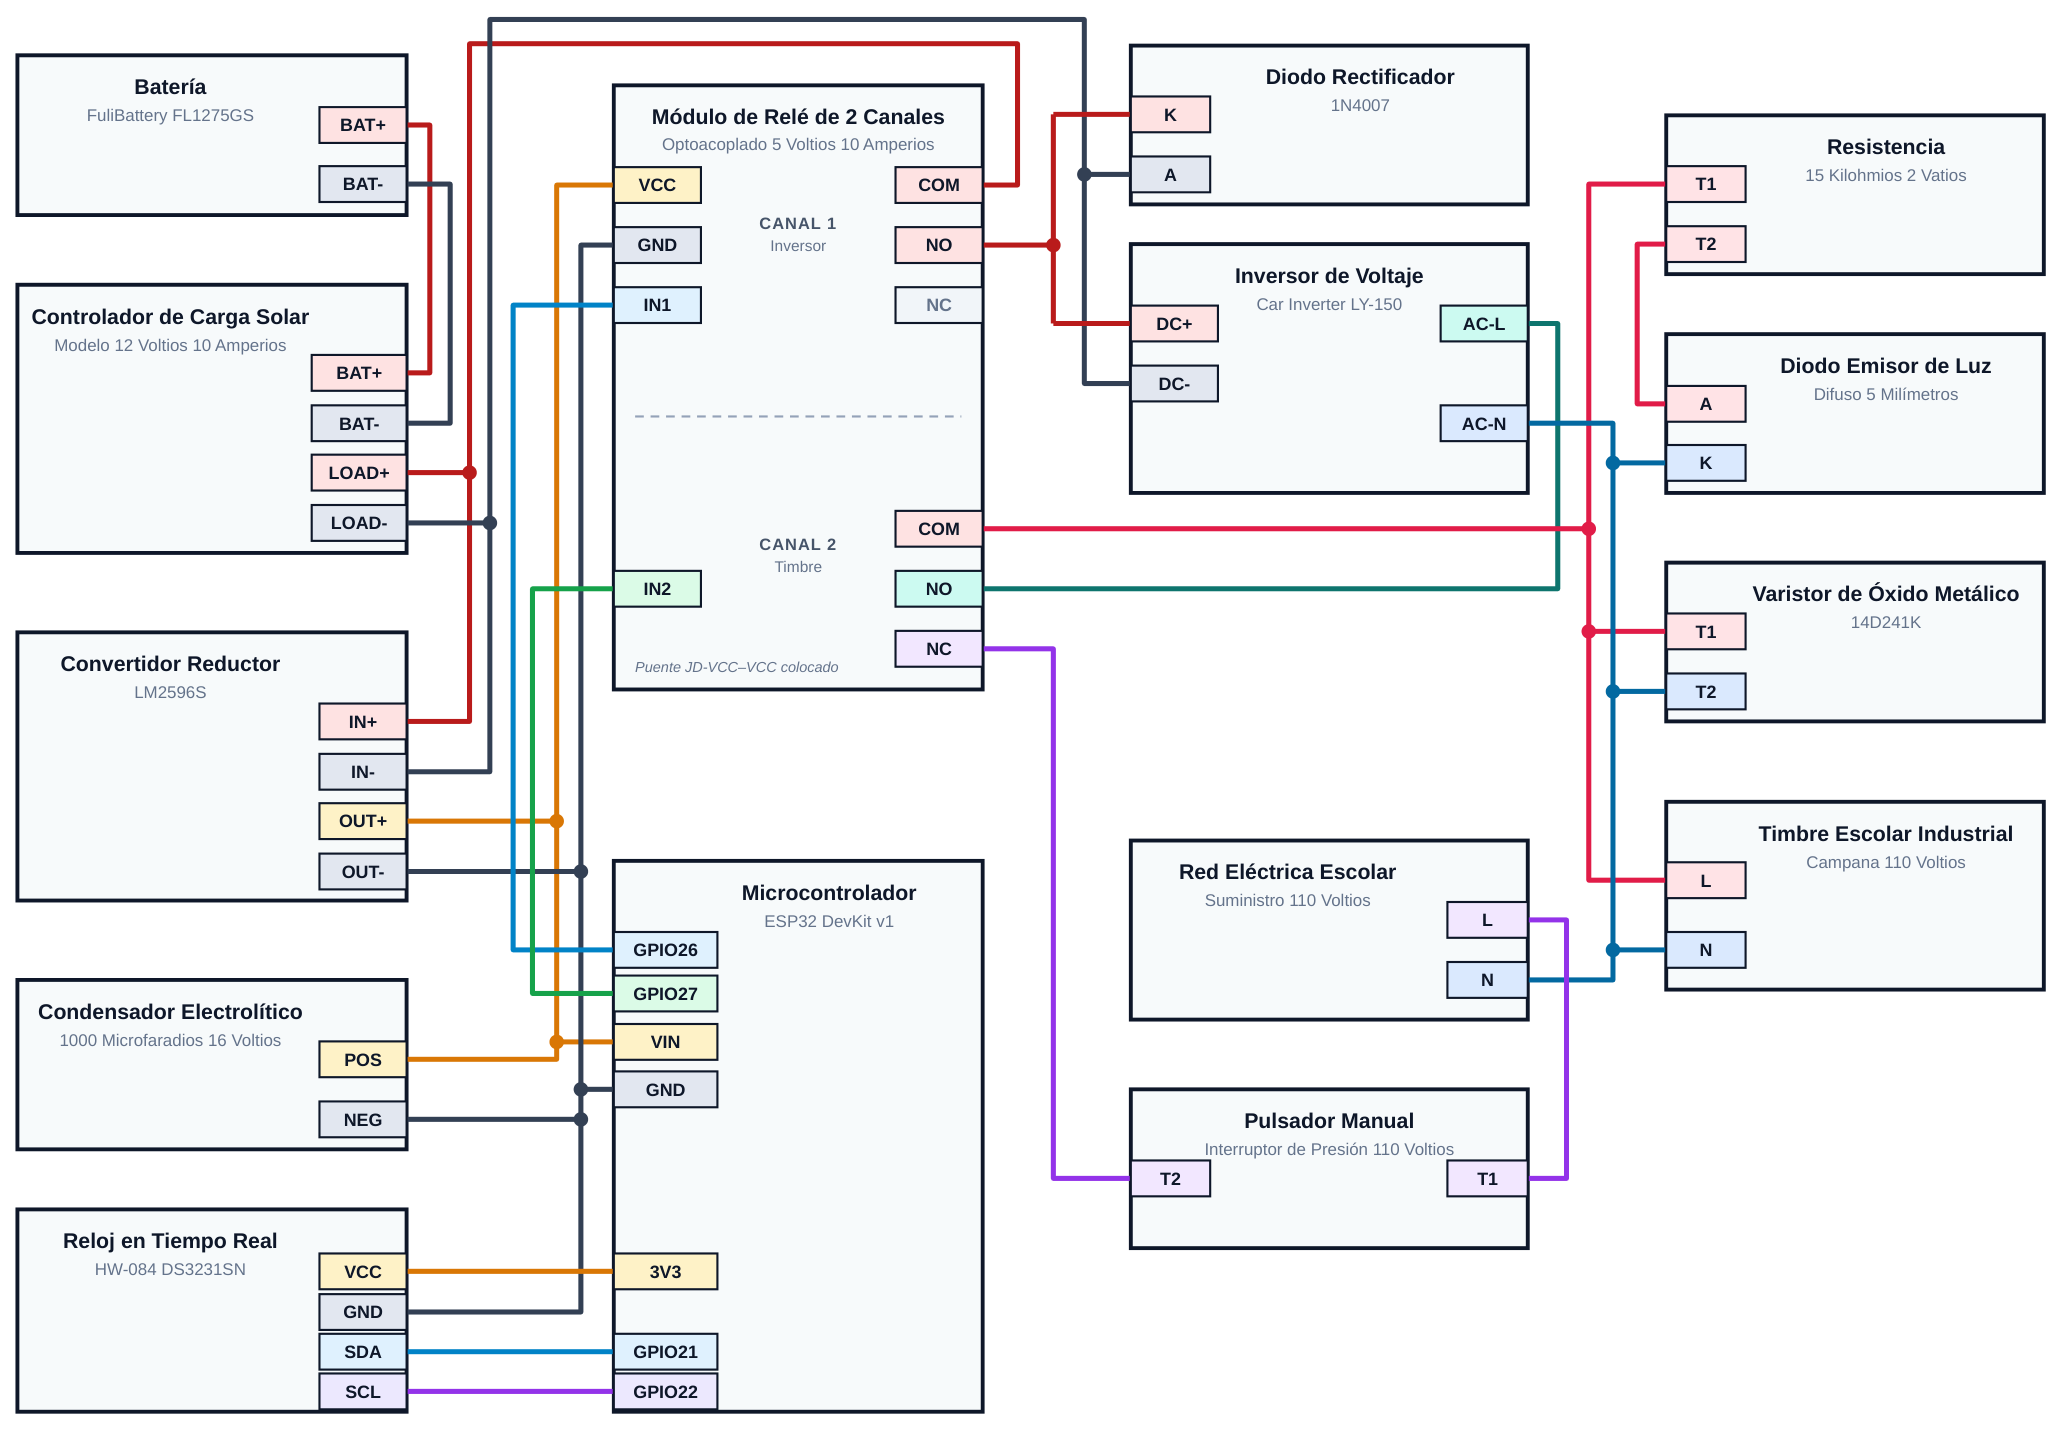
\includegraphics[width=\linewidth]{figuras/esquema-electrico.png}
\caption{Circuito de SolarBell con módulo de relé doble}
\label{fig:esquema}
\fuente{Detalle del diagrama eléctrico del proyecto \cite{diagrama}.}
\end{figure}

\begin{table}[H]
\centering\small
\caption{Identificación de los contactos de potencia}
\begin{tabularx}{\linewidth}{@{}P{2.95cm}YY@{}}
\toprule
\textbf{Canal} & \textbf{En reposo} & \textbf{Durante la activación} \\
\midrule
Canal 1 & El contacto normalmente abierto deja la entrada positiva del inversor sin alimentación de la salida de carga. & Se cierra la ruta de 12\,V hacia el inversor durante la secuencia. \\
Canal 2 & El contacto normalmente cerrado deja disponible la ruta de la red escolar a través del pulsador. & El contacto normalmente abierto selecciona la línea del inversor para cada toque. \\
\bottomrule
\end{tabularx}
\end{table}

\nota{\textbf{Revisión de la conmutación.} El diagrama representa un neutro común entre la red escolar y la salida del inversor. Antes de intervenir o reproducir el circuito, el personal competente debe revisar esa configuración para el inversor y la instalación reales, así como la capacidad de los contactos, el aislamiento, la puesta a tierra y las protecciones aplicables \cite{diagrama,retie}.}

\clearpage
\section{Puesta en servicio y configuración}
\label{sec:servicio}
\subsection{Condiciones previas}
Coordine con el colegio una franja de prueba que no interrumpa las clases. Si hubo una instalación o un cambio en el circuito, solicite al responsable eléctrico la revisión del gabinete, la sujeción y el rotulado, las protecciones y la conmutación de fuentes. El responsable autoriza la energización y determina las verificaciones aplicables \cite{retie}. Realice la configuración de software con el gabinete cerrado, salvo la carga del firmware, que requiere acceso al puerto USB del ESP32 y la autorización del responsable eléctrico.

\subsection{Configuración y carga del firmware}
\label{sec:firmware}
El firmware está en \pin{ESP32/solarbell\_local/solarbell\_local.ino}. Las opciones de cada instalación van en \pin{configuracion.h}, que no se publica con el código porque contiene la clave de la red \cite{repo}.

\begin{enumerate}
  \item Copie \pin{configuracion.ejemplo.h} como \pin{configuracion.h} en la misma carpeta.
  \item Defina \pin{RED\_CLAVE} con al menos 8 caracteres. Con una clave más corta, el ESP32 no puede crear la red SolarBell. Esa clave es la única protección del sistema: quien la conozca puede cambiar el horario y tocar la campana.
  \item Active las opciones de la instalación quitando el comentario de cada línea: \pin{USAR\_DS3231} para el reloj, \pin{PIN\_RELE 27} para la campana, \pin{PIN\_INVERSOR 26} para el inversor y \pin{PIN\_INTERRUPTOR\_WIFI 33} para el interruptor. Si el módulo de relés se activa en bajo, active también \pin{RELE\_ACTIVO\_EN\_BAJO} e \pin{INVERSOR\_ACTIVO\_EN\_BAJO}. Sin \pin{PIN\_RELE}, el firmware solo simula los toques con el LED.
  \item En Arduino IDE, instale el núcleo \textbf{esp32} de Espressif y elija la placa \textit{ESP32 Dev Module} con el esquema de particiones por defecto, que reserva la partición para LittleFS. Instale las librerías \textbf{ArduinoJson} (versión 7) y \textbf{RTClib} de Adafruit.
  \item Compile y suba el programa por USB. También puede usar \pin{arduino-cli compile --fqbn esp32:esp32:esp32 solarbell\_local} y \pin{arduino-cli upload}.
  \item Abra el monitor serie a 115.200 baudios. El equipo informa la red creada, la unión a la red del colegio y cada toque.
  \item Desde la aplicación, en la pestaña \textbf{Campana}, confirme la versión 0.8.0.
\end{enumerate}

\nota{\textbf{Qué se conserva al actualizar.} Subir el firmware no borra la partición de datos, salvo que se active en Arduino IDE la opción de borrar toda la flash antes de subir: el horario, el historial y la red del colegio se conservan. Un horario guardado por la versión 0.2, en segundos, se convierte a milisegundos al arrancar. Antes de actualizar, consulte el horario en la aplicación para tener una referencia.}

La aplicación se compila desde \pin{frontend/} con \pin{bun run apk}, que requiere JDK 21 y el SDK de Android, y genera un APK de depuración para Android 7.0 o posterior \cite{repo}.

\subsection{Conexión y comprobación del reloj}
\begin{enumerate}
  \item Compruebe que el sistema esté disponible y que el interruptor de Wi-Fi esté abierto, de modo que exista la red SolarBell. En el teléfono, revise fecha, hora y zona horaria antes de conectarse, porque la aplicación transmite esa referencia al equipo.
  \item Conecte el teléfono Android a la red \textbf{SolarBell}, con la clave definida en \pin{RED\_CLAVE}, o a la red del colegio elegida desde la aplicación. Ambas rutas son locales y funcionan sin acceso a Internet. En la red propia, el equipo está en \pin{192.168.4.1}. En la red del colegio, la aplicación lo encuentra sola por su última IP, por \pin{solarbell.local} o recorriendo la subred.
  \item Abra la aplicación y consulte la pestaña \textbf{Campana}. Verifique \textbf{Conectada}, \textbf{En hora} y firmware 0.8.0. Al conectarse, la aplicación corrige la hora del equipo si difiere en más de 5\,s. Compare la vista del día con la fecha y la hora local.
  \item Para operar desde otro punto del colegio, en \textbf{Campana}, tarjeta \textbf{Wi-Fi de casa}, elija una red de 2,4\,GHz y escriba su clave. La red solo queda guardada si el equipo obtiene una IP. Si falla en 20\,s, vuelve a la red anterior.
\end{enumerate}

\subsection{Programación, consulta y orden inmediata}
\begin{enumerate}
  \item \textbf{Horario semanal.} Revise los timbres existentes. Para cada cambio, defina nombre, hora, cantidad de toques, duración y pausa, o una duración propia para cada toque y pausa. El horario semanal se aplica de lunes a viernes; la aplicación muestra esos días pero no los cambia. Para modificar un día concreto, use una fecha especial. Cada cambio se guarda en el equipo al confirmarlo.
  \item \textbf{Fecha especial.} Seleccione la fecha y elija \textbf{Horario especial}, con sus timbres propios, o \textbf{Sin timbrado}. La fecha especial reemplaza el horario ordinario de ese día. Revise el próximo timbre y la cuenta regresiva en la vista del día.
  \item \textbf{Toque inmediato.} En una franja acordada, seleccione un patrón y envíe la orden. Use la opción de detener el toque si necesita interrumpir la prueba. Compare el resultado audible con la pestaña \textbf{Historial}, donde el ESP32 anota cada toque al terminar como completo, detenido o cortado.
\end{enumerate}

\nota{\textbf{Cambios sin conexión.} Un cambio efectuado fuera de alcance no se guarda en la campana: la aplicación vuelve al último horario confirmado. Restablezca la conexión y repita la edición. Con la radio apagada, la programación guardada sigue ejecutándose \cite{fichas,informe,repo}.}

Tras una intervención, restaure los horarios y las excepciones autorizados. Consulte el próximo aviso en Android y retire los eventos temporales de prueba.

\clearpage
\section{Comprobaciones de funcionamiento}
\label{sec:pruebas}
Aplique estas comprobaciones al entregar el sistema y después de cambios que afecten su operación. Anote la hora prevista, el resultado audible y el registro del historial. El ESP32 anota cada toque al terminar, con el tiempo que sonó; el historial prueba la orden, no el sonido, así que la respuesta acústica se comprueba en el lugar de uso \cite{informe,fichas,repo}.

\begin{table}[H]
\centering\small
\caption{Verificaciones de servicio}
\begin{tabularx}{\linewidth}{@{}P{3.05cm}YY@{}}
\toprule
\textbf{Comprobación} & \textbf{Acción de prueba} & \textbf{Resultado esperado} \\
\midrule
Hora y calendario & Conectar Android y volver a consultar un cambio de horario. & Fecha y hora coherentes y evento recuperado del ESP32. \\
Timbrado programado & Guardar un aviso cercano y observar la ejecución y el historial. & Aviso a la hora definida, patrón correcto y registro \textbf{Programado}, \textbf{Completo}, en \textbf{Historial}. \\
Fecha especial & Consultar una fecha con programación propia o sin timbres. & La agenda de esa fecha refleja la excepción. \\
Toque y detención & Iniciar un toque desde Android e interrumpirlo desde la app. & La salida se activa, la orden de detención interrumpe el toque y el historial lo muestra como \textbf{Detenido}. \\
Ahorro de radio & Con la red del colegio guardada, cerrar el interruptor de Wi-Fi y esperar un timbre de prueba. & La red SolarBell desaparece, la app sigue respondiendo desde la red del colegio y el horario se ejecuta. \\
Operación autónoma & Sin red del colegio guardada, cerrar el interruptor para apagar el Wi-Fi y esperar un timbre de prueba. & El teléfono pierde el enlace y el horario local se ejecuta. Al abrir el interruptor, el toque aparece en el historial. \\
Pérdida de alimentación & Con autorización, cortar la alimentación del control y restablecerla. & Con DS3231, el reloj sigue \textbf{En hora} y el horario continúa. Sin DS3231, el LED parpadea hasta que un teléfono se conecte. \\
Pulsador de pared & Con el timbre en reposo y la red escolar disponible, accionar el pulsador. & La campana responde a la pulsación. \\
\bottomrule
\end{tabularx}
\end{table}

\begin{figure}[H]
\centering
\begin{minipage}[c]{0.41\linewidth}
  \centering
  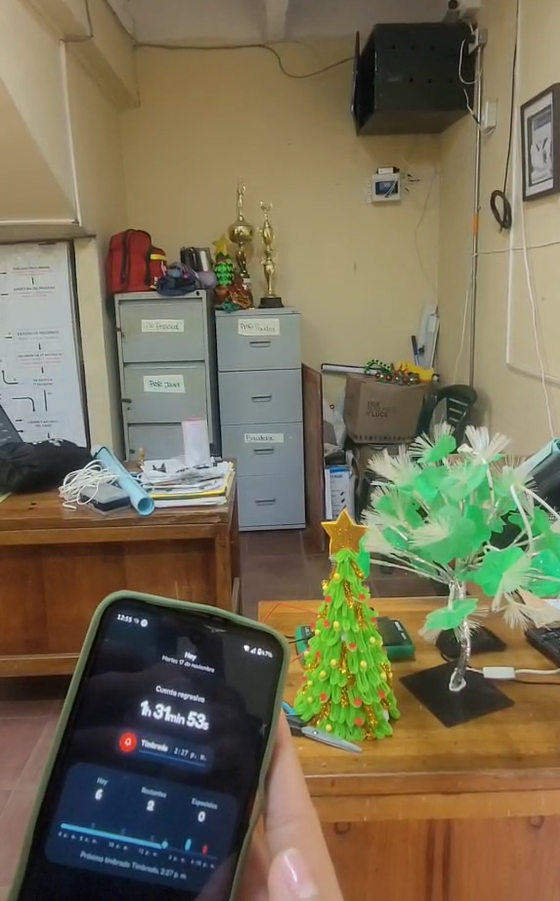
\includegraphics[width=0.83\linewidth]{figuras/prueba-en-sitio.png}
\end{minipage}\hfill
\begin{minipage}[c]{0.55\linewidth}
  \raggedright
  \textbf{Verificación en Cecilia de Lleras}\par\smallskip
  El equipo reportó que el ESP32 ejecutó el aviso a la hora programada en la institución. La fotografía se tomó antes del timbrado y muestra la cuenta regresiva para el aviso de las 2:27\,p.\,m. \cite{informe}.
\end{minipage}
\caption{Vista de la aplicación durante la prueba en sitio}
\end{figure}

\clearpage
\section{Diagnóstico}
\label{sec:diagnostico}
Empiece por comprobar el estado de la aplicación, la agenda del día y el historial, con el gabinete cerrado. Al reportar una falla, indique si el aviso era programado, inmediato desde Android o accionado con el pulsador de pared.

\begin{table}[H]
\centering\small
\caption{Síntomas y acciones de diagnóstico}
\begin{tabularx}{\linewidth}{@{}P{3.44cm}YY@{}}
\toprule
\textbf{Síntoma} & \textbf{Comprobación inicial} & \textbf{Acción} \\
\midrule
La app muestra el equipo fuera de alcance. & Confirmar la posición del interruptor de Wi-Fi y que el teléfono use la red SolarBell o la del colegio configurada en el equipo. Con el interruptor cerrado no existe la red SolarBell. & Volver a conectar y pulsar \textbf{Buscar campana}. Si persiste, revisar el monitor serie por USB y escalar la revisión de la red o de la alimentación del control. \\
La red SolarBell no aparece con el interruptor abierto. & La longitud de \pin{RED\_CLAVE} en \pin{configuracion.h}. & Usar una clave de 8 caracteres o más y volver a subir el firmware. \\
El LED azul parpadea lento. & El equipo no tiene hora. & Conectar un teléfono con la hora correcta. Si ocurre tras cada corte, revisar el DS3231, su batería y la opción \pin{USAR\_DS3231}. \\
Historial muestra «No se pudo leer el historial» con el equipo conectado. & La versión de firmware en \textbf{Campana}. & El historial existe desde la versión 0.8.0. Actualizar el firmware (sección~\ref{sec:firmware}). \\
Un cambio de horario no aparece. & Revisar el enlace y volver a consultar el calendario guardado. & Repetir la edición solo cuando el equipo esté al alcance. Confirmar el cambio con una lectura posterior. \\
El aviso suena a otra hora o no está en la agenda. & Revisar la hora y la zona del teléfono, el estado del reloj, el día de la semana, las fechas especiales y el historial. & Corregir la hora del teléfono y reconectar la app. Si el reloj pierde la hora después de un corte, solicitar revisión del RTC y su respaldo. \\
Hay un timbrado en el historial, pero no se oyó la campana. & Registrar el origen del aviso y comparar hora, patrón y respuesta en el lugar. & Solicitar revisión de la etapa de potencia y de la campana por personal competente. \\
El timbre se activa fuera de la programación. & Comparar agenda, fechas especiales e historial. Un registro \textbf{Manual} indica una orden desde la app; sin registro, el origen pudo ser el pulsador de pared o una falla de conmutación. & Suspender las pruebas y registrar el caso. Si se repite, solicitar revisión del mando y de los relés. \\
El pulsador no acciona la campana. & Confirmar que el sistema esté en reposo y consultar si hay suministro en el circuito escolar. & Derivar la revisión del pulsador, el contacto de reposo y la carga al responsable eléctrico. \\
El control se reinicia durante el timbrado. & Registrar si el reinicio coincide con el comienzo del toque o con la conmutación. & Solicitar revisión de batería, alimentación regulada y transitorios bajo las condiciones autorizadas de ensayo. \\
\bottomrule
\end{tabularx}
\end{table}

\nota{\textbf{Si hay indicios de falla eléctrica.} Ante olor a quemado, humo, sobrecalentamiento o daño del gabinete, suspenda el uso y mantenga el área despejada. Avise al responsable del colegio para que personal competente aísle y evalúe el equipo \cite{retie}.}

\clearpage
\section{Mantenimiento y entrega técnica}
\label{sec:mantenimiento}
\begin{table}[H]
\centering\small
\caption{Actividades de mantenimiento}
\begin{tabularx}{\linewidth}{@{}P{3.45cm}YY@{}}
\toprule
\textbf{Cuándo} & \textbf{Actividad} & \textbf{Registro} \\
\midrule
Al cambiar el calendario escolar & Revisar horarios, fechas especiales y próximo aviso. & Programación aprobada y fecha de aplicación. \\
Después de un corte o reinicio & Verificar estado del RTC, horario guardado y próximo evento. Si corresponde, reconectar Android para actualizar la hora. & Estado del equipo y resultado de un aviso de prueba. \\
En la revisión preventiva & Inspeccionar desde el exterior limpieza, sujeción y estado visible del panel y del gabinete. Solicitar al personal competente la revisión de batería y protecciones. & Condición observada, responsable y acción tomada. \\
Tras cambiar un componente o el firmware & Conservar una copia de consulta del horario vigente y registrar versiones. Repetir las comprobaciones que afecte el cambio. & Componente o versión anterior y nueva, pruebas y resultado. \\
Cada trimestre & Consultar el historial si se necesita conservarlo. Guarda unos 1.000 toques, unos cuatro meses y medio con diez avisos diarios, y descarta solo los más antiguos. & Capturas o notas de los periodos que el colegio quiera conservar. \\
\bottomrule
\end{tabularx}
\end{table}

\textbf{Información para soporte.} Anote fecha, versión visible en Android, origen del timbrado, hora esperada y observada, patrón, respuesta audible, registro en la app y diagnóstico. Adjunte la evidencia pertinente y documente quién verificó la recuperación del servicio.

\textbf{Retiro y retorno al servicio.} Informe al colegio antes de interrumpir los avisos y acuerde cómo se anunciarán los cambios de clase durante la intervención. Al restablecer el servicio, confirme la hora, el calendario y un timbrado de prueba. Registre el resultado y comunique el retorno a la operación.

\textbf{Archivos para la entrega.} Conserve el esquema de la instalación, la ficha técnica, la programación autorizada, el APK y el \pin{configuracion.h} de la placa instalada, guardado fuera del repositorio porque contiene la clave. Las rutas HTTP del equipo y la persistencia en la flash se describen en la sección 5.2 del informe y en \pin{ESP32/README.md}. El procedimiento de actualización está en la sección~\ref{sec:firmware} \cite{informe,fichas,repo}.

\textbf{Revisión eléctrica.} El responsable competente determina la documentación, las firmas y la evaluación de conformidad aplicables al sitio. Mantenga con la instalación los planos finales y el registro de las intervenciones autorizadas \cite{retie}.

\section{Fuentes}
\begingroup
\small
\renewcommand{\section}[2]{}
\begin{thebibliography}{9}
\setlength{\itemsep}{3pt}
\bibitem{informe} Equipo SolarBell. (2026). \textit{SolarBell: sistema de timbre automatizado con energía solar. Informe final del Proyecto de Aula Semestral}. Universidad de Córdoba. Secciones 5.2 y 5.3.
\bibitem{fichas} Equipo SolarBell. (2026). \textit{Fichas de hardware y software. SolarBell}. Universidad de Córdoba.
\bibitem{diagrama} Equipo SolarBell. \textit{Circuito del sistema de timbre escolar: relé doble}. Diagrama del prototipo.
\bibitem{repo} Equipo SolarBell. (2026). \textit{SolarBell}, rama \pin{main}, revisión \pin{0adeb14}: firmware 0.8.0 y aplicación Android. \href{https://github.com/AndresOrtizJDK/SolarBell/tree/0adeb14514f4e0b15457052f21800002322fbb43}{Repositorio en GitHub}.
\bibitem{retie} Ministerio de Minas y Energía de Colombia. (2026). \textit{Reglamento Técnico de Instalaciones Eléctricas, Resolución 40284 del 23 de junio de 2026}. \href{https://minenergia.gov.co/documents/16522/Resolucion-40284-23062026-compilada.pdf}{Resolución compilada}, Libro 1 y Libro 3, artículo 3.2.2.
\end{thebibliography}
\endgroup
\end{document}
